%%%%%%%%%%%%%%%%%%%%%%%%%%%%%%%%%%%%%%%%%%%%%%%%%%%%%%%%%%%%%%%%%
% Dissertacao de Mestrado / Dept Fisica, CFM, UFSC              %
% Andre@UFSC - 2011                                             %
%%%%%%%%%%%%%%%%%%%%%%%%%%%%%%%%%%%%%%%%%%%%%%%%%%%%%%%%%%%%%%%%%

%:::::::::::::::::::::::::::::::::::::::::::::::::::::::::::::::%
%                                                               %
%                          Capítulo 3                           %
%                                                               %
%:::::::::::::::::::::::::::::::::::::::::::::::::::::::::::::::%

%***************************************************************%
%                                                               %
%                         Crossmatch                            %
%                                                               %
%***************************************************************%

\chapter{Crossmatch entre SDSS/STARLIGHT e GALEX}
\label{sec:Crossmatch}

% TODO: Crossmatch - intro

\section{Bancos de dados}
% TODO: O Que são bancos de dados?

\subsection{CasJobs}
% TODO: Apresentar o Casjobs.


\section{Banco de dados do STARLIGHT}
% TODO: Construção do banco de dados do starlight.
Starlight gera dados em arquivos texto. São gigabytes de dados. Tratável para
uso pessoal, mas não é muito viável a distribuição.

Importação para o sql server. 

\subsection{Estrutura do banco de dados}
% TODO: Estrutura banco de dados do starlight.

% TODO: Adicionar figura - esquema BD starlight.
\begin{figure}
	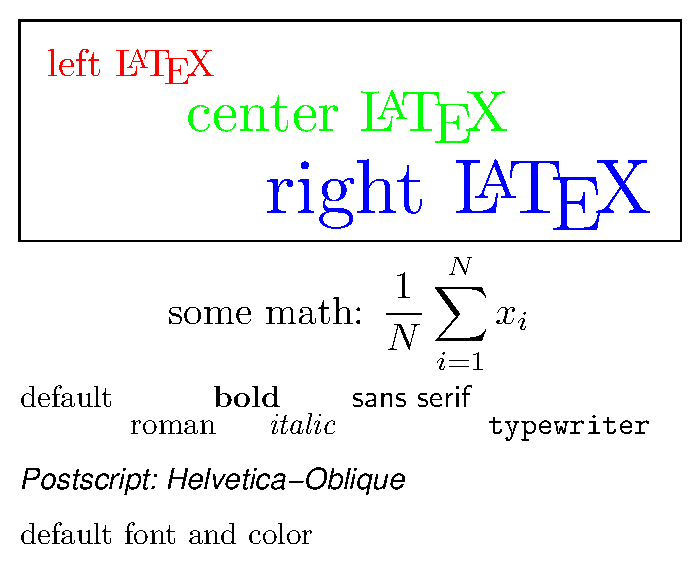
\includegraphics[width=0.5\textwidth]{figuras/test.eps}
	\caption[Esquema do banco de dados do \starlight.]
	{Esquema do banco de dados do \starlight.}
	\label{fig:EsquemaBDStarlight}
\end{figure}

\subsection{Amostra do STARLIGHT}
\label{sec:Crossmatch:AmostraStarlight}
% TODO: Definir a amostra inicial do starlight.

% FIXME: Explicar o que é uma chave primária.
A amostra de galáxias do \starlight contém $926246$ espectros do \SDSS. A
identificação de cada espectro é feita através de um tripleto: a data juliana
média da observação ({\tt MJD}, {\em Mean Julian Date}), a identificação da
placa de suporte das fibras ópticas ({\tt Plate}) e a identificão da fibra
utilizada para a obtenção do espectro ({\tt FiberID}). Este tripleto ({\tt MJD},
{\tt Plate}, {\tt FiberID}) identifica unicamente um espectro. Porém, é mais
conveniente (e eficiente) ter um identificador único{\footnote{Chave primária
\fixme}} para os registros num banco de dados. No caso do \SDSS, a tabela de
espectros ({\tt SpecObjAll}) tem um identificador chamado {\tt SpecObjID}.

% TODO: Adicionar figura - esquema simplificado da BD do SDSS.
\begin{figure}
	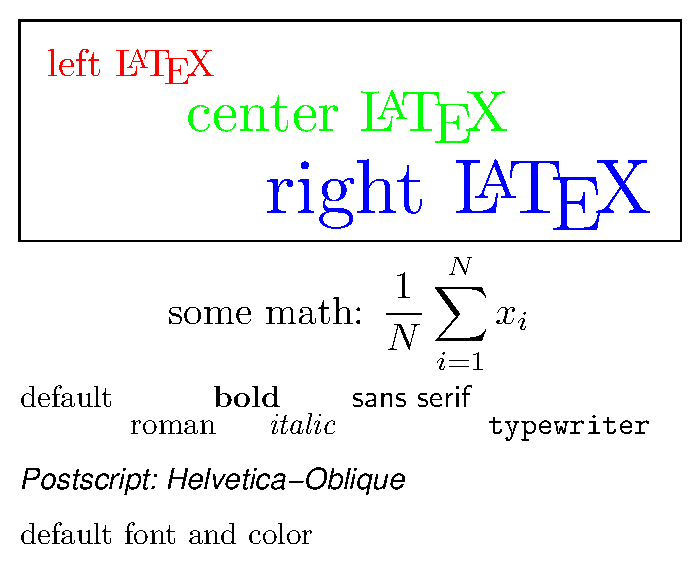
\includegraphics[width=0.5\textwidth]{figuras/test.eps}
	\caption[Esquema do banco de dados do \SDSS.]
	{Esquema do banco de dados do \SDSS.}
	\label{fig:EsquemaSDSS}
\end{figure}

% FIXME: Citação para cobertura do céu do SDSS.
Além de espectros, o banco de dados do \SDSS (figura \ref{fig:EsquemaSDSS})
contém fotometria de $1/4$ do céu.\citneed Os objetos com dados de fotometria
também tem um identificador único, {\tt ObjID}. Existe uma coluna na tabela de
espectros chamada {\tt BestObjID}, que aponta para o registro de fotometria
(tabela {\tt PhotoObjAll}) mais provável para cada espectro. É importante
salientar que nem todo espectro tem um {\tt BestObjID} definido.

A tabela de índices da amostra de galáxias do \starlight (esquema na figura
\ref{fig:TabelaAmostraStarlight}) contém inicialmente os tripletos [{\tt MJD},
{\tt Plate}, {\tt FiberID}]. Dentro do ambiente {CasJobs} do \SDSS
DR7\footnote{{\em CasJobs} \SDSS DR7 - \url{http://casjobs.sdss.org/CasJobs/}} a
tabela tem os valores de {\tt SpecObjID} e {\tt BestObjID} prenchida através da
execução da {\em query} mostrada na figura \ref{fig:AtualizaObjIds}. Entre os
objetos na amostra do \starlight, $622$ objetos não tem a sua contraparte
fotométrica.

% TODO: Adicionar figura - Tabela amostra do starlight.
\begin{figure}
	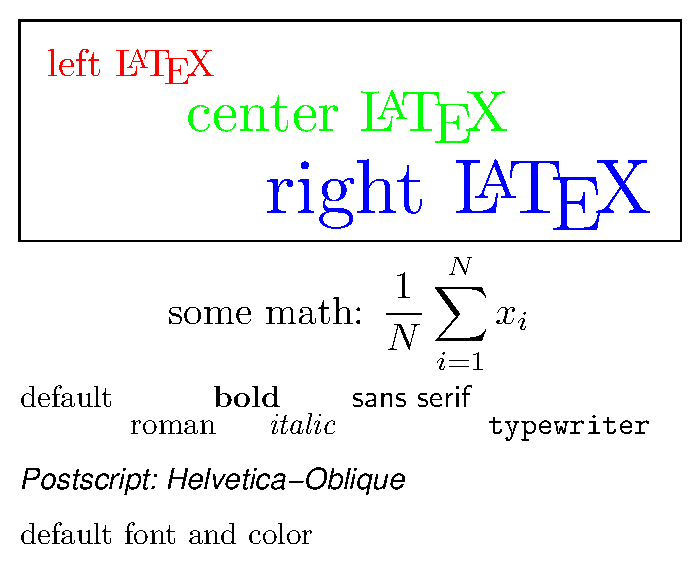
\includegraphics[width=0.5\textwidth]{figuras/test.eps}
	\caption[Esquema da tabela de índices da amostra do \starlight.]
	{Esquema da tabela de índices da amostra do \starlight. Os tipos de dados são
	referentes à implementação do banco de dados.}
	\label{fig:TabelaAmostraStarlight}
\end{figure}

\begin{figure}
	\begin{Verbatim}[commandchars=\\\{\}]
	\textbf{UPDATE} sample
		\textbf{SET} SpecObjID=so.SpecObjID, ObjID=so.BestObjID
	\textbf{FROM} sample s2 \textbf{INNER JOIN} DR7..SpecObjAll so
		\textbf{ON} so.MJD=s2.MJD
		\textbf{AND} so.Plate=s2.Plate
		\textbf{AND} so.FiberID=s2.FiberID
	\end{Verbatim}
	\caption
	[{\em Query} para atualizar os índices da amostra de galáxias do
	\starlight.]
	{Atualização dos índices da amostra de galáxias do \starlight. A {\em query}
	foi executada no {\em CasJobs} do \SDSS DR7 para obter {\tt SpecObjID} e {\tt
	BestObjID} dado o tripleto [{\tt MJD}, {\tt Plate}, {\tt FiberID}].}
	\label{fig:AtualizaObjIds}
\end{figure}


\section{Crossmatch SDSS/GALEX}
% TODO: Crossmatch SDSS/GALEX.
\cite{Budavari2009}.

\subsection{Indexação HTM}
% TODO: Indexação HTM.

\subsection{Análise de completeza}
% TODO: Análise de completeza do crossmatch SDSS/GALEX 


\section{Definição das amostras SDSS/STARLIGHT e GALEX}
\label{sec:Crossmatch:DefAmostras}
% TODO: Definição das amostras a serem usadas no próximo cap. (MGS e LRG).

% TODO: Como foi feito o match.

% TODO: Adicionar figura - tabela xSDSSDR7.
\begin{figure}
	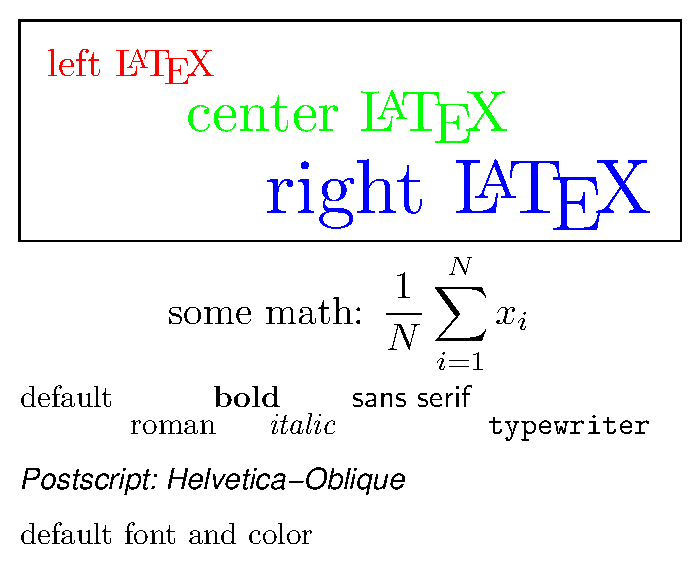
\includegraphics[width=0.5\textwidth]{figuras/test.eps}
	\caption[Esquema da tabela de {em crossmatch} entre objetos do \galex e do
	\SDSS.]
	{Esquema da tabela de {\em crossmatch} entre objetos do \galex e do
	\SDSS.}
	\label{fig:TabelaxSDSSDR7}
\end{figure}

% FIXME: Corrigir caption da figura do match AIS.
\begin{figure}
	\begin{Verbatim}[commandchars=\\\{\}]
	\textbf{SELECT INTO} mydb..galex_ais
		s.objid \textbf{AS} sdssobjid, x.objid \textbf{AS} galexobjid,
		s.mjd, s.plate, s.fiberid,
		g.nuv_mag, nuv_magErr,
		g.fuv_mag, g.fuv_magErr,
		g.e_bv,
		g.band,
		x.distance,
		pe.nexptime,
		pe.fexptime
	\textbf{FROM} mydb..sample s
	\textbf{LEFT JOIN} xSDSSDR7 x
		\textbf{ON} s.objid = x.sdssobjid
		\textbf{AND} x.distanceRank=1
		\textbf{AND} x.reverseDistanceRank=1
		\textbf{AND} x.multipleMatchCount=1
		\textbf{AND} x.reverseMultipleMatchCount=1
	\textbf{LEFT JOIN} photoobjall g
		\textbf{ON} g.objid = x.objid
	\textbf{LEFT JOIN} photoextract e
		\textbf{ON} e.photoextractid=g.photoextractid
	\textbf{WHERE} e.mpstype='AIS'
	\end{Verbatim}
	\caption[{\em Query} para o {\em match} entre os objetos da amostra do
	\starlight e \galex AIS.]
	{{\em Query} para o {\em match} entre os objetos da amostra do \starlight e
	\galex AIS. A mesma {\em query} foi usada para o MIS, trocando apenas o nome da
	tabela para {\tt galex\_mis} e modificando a última linha para {\tt
	e.mpstype='MIS'}.}
	\label{fig:QueryMatchAIS}
\end{figure}


% TODO: Alguma estatística.


\section{Correções na fotometria UV}
\label{sec:Crossmatch:Correcoes}

\subsection{K-correct}
% TODO: K-correction

\subsection{Poeira}
% TODO: Correção por poeira etc.


%% End of this chapter
